\section{Periféricos Principales}
\label{sec:perif}

\begin{itemize}
\item Placa conversora USB a Serie: es necesaria para poder conectar a una computadora via puerto USB y que la computadora sea capaz de reconocer al dispositivo como un puerto serie virtual. De esta manera es posible utilizar las funciones de Matlab que permiten enviar datos a través de un puerto serie. Además estas placas incluyen conexiones para alimentar al microcontrolador con lo cual se lo podría energizar solamente con la conexión a una computadora sin necesidad de utilizar un cable adicional. En el mercado argentino se encuentran este tipo de placas basadas en dos integrados distintos: Cp2102 y CH340, cuyas correspondientes hojas de datos se incluyen a continuación:
\begin{itemize}
\item \href{https://www.olimex.com/Products/Breadboarding/BB-CH340T/resources/CH340DS1.PDF}{\color{blue} Hoja de datos CH340}
\item \href{https://www.sparkfun.com/datasheets/IC/cp2102.pdf}{\color{blue} Hoja de datos Cp2102}
\end{itemize}

\begin{figure}[H]
  \centering
  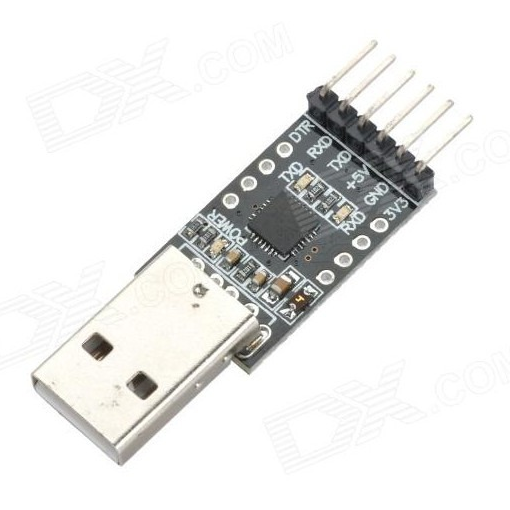
\includegraphics[width=0.6\textwidth]{images/conversor_usbttl.png}
  \caption{Ejemplo de placa conversora usb a serie}
  \label{fig:usbattl}
\end{figure}

\item Parlante o Altavoz: Necesario para poder generar el desplazamiento en el espejo. Será necesario evaluar distintos tipos de parlantes para entender cuál resulta útil para cumplir nuestros objetivos.
\item Diseñar un soporte para el dispositivo en su totalidad de manera tal que pueda ser utilizado en una mesa antivibratoria en la cual se encuentra instalado el interferómetro. En este soporte estará colocado el parlante con un espejo pegado al mismo.
\end{itemize}